\section{Experimentálne overenie funkčnosti riešenia}

Tato kapitola je venovaná overeniu správnosti implementácie. Boli vykonané nasledujúce štyri experimenty, 
ktoré mali potvrdiť, alebo vyvrátiť správnu funkčnosť riešenia. 
\begin{enumerate}
 \item \textbf{Prvý test} overil konektivitu a prenos údajov medzi exportérom a mediátorom a následne medzi 
 mediátorom a kolektorom.
 \item \textbf{Druhy test} porovnal hodnoty údajov exportovaných mybeem-om s hodnotami uloženými v databáze po prechode
 cez Mediátor bez sprostredkovateľského procesu.
 \item \textbf{Tretí test} demonštroval správnosť anonymizácie údajov v podaní sprostredkovateľského procesu 
 \verb|ExampleProcess|, spomínaného vyššie v návrhu a implementácii.
 \item \textbf{Štvrtý test} bol tzv. záťažovým testom, overoval stabilitu Mediátora pri dlhodobom behu a 
 pri spracovávaní prevádzky s vysokým počtom tokov.
\end{enumerate}

%%%%%

\subsection{Testovacia topológia}

Pri všetkých testoch bol použitý virtualizačný nástroj VirtualBox, v ktorom boli vytvorené tri virtuálne 
počítače, zapojené do topológie, ktorú možno vidieť na Obrázku \ref{o:test_topologia}.
Na všetkých troch počítačoch sa používal operačný systém Ubuntu 12.04 LTS v desktopovej verzii. Na prvom 
počítači bol nainštalovaný exportér mybeem (verzia 1.1-6 s podporou pre IPFIX Mediátor), ktorý exportoval 
správy druhému počítaču na UDP port vyhradený pre IPFIX komunikáciu - \emph{4739}. Tam bežal Mediátor
verzie 1.0. Ten zase preposielal správy na tretí počítač (taktiež port \emph{4739}), kde bol spustený 
kolektor JXColl (verzia 3.9) s funkčnou PostgreSQL databázou. Počítače boli zapojené v jednej lokálnej 
sieti a všetky mali prístup na Internet.

\begin{figure}[ht!]
\centering
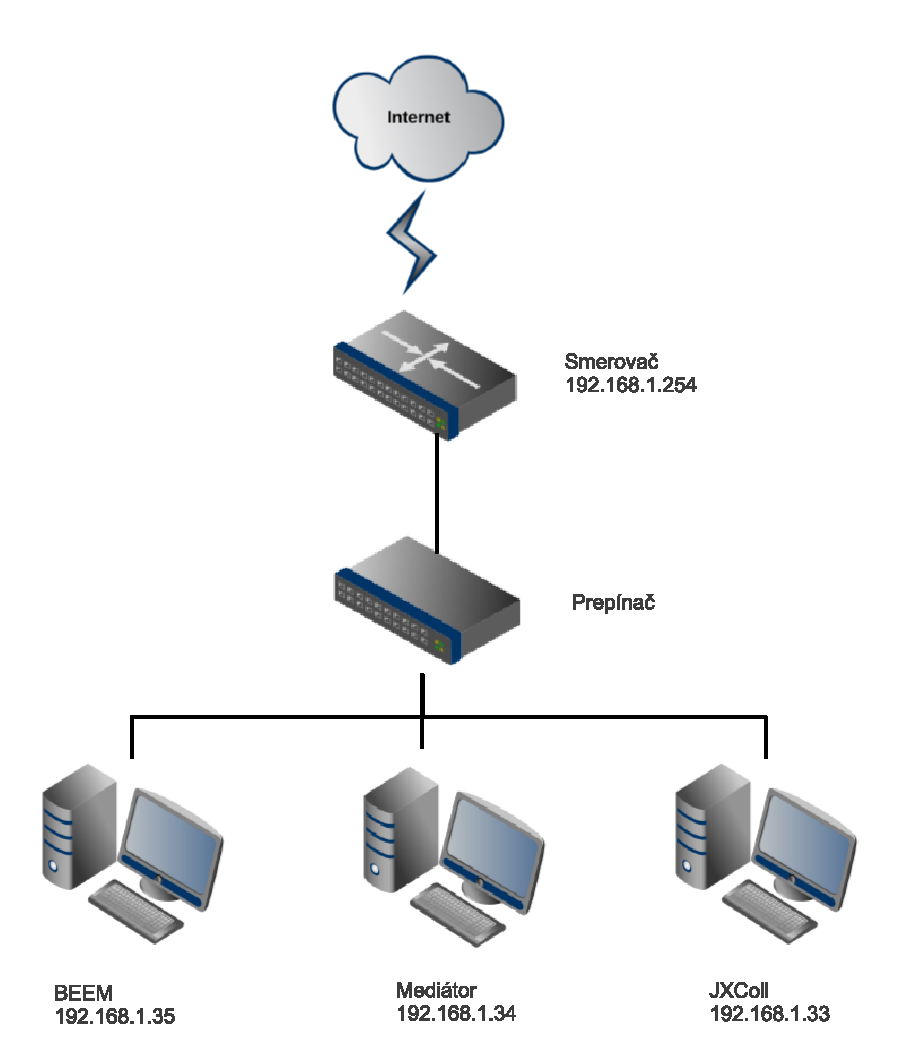
\includegraphics[width=0.8\textwidth]{test_topologia}
\caption{Testovacia topológia}\label{o:test_topologia}
\end{figure}

%%-------------------------

\subsection{Test konektivity}

Prvý experiment overoval základnú konektivitu medzi exportérom a kolektorom v prípade, že je medzi ne 
zaradený mediátor. Vo svojej východiskovej konfigurácii vypisuje mybeem logovacie správy na štandardný 
výstup. Tie obsahujú základné informácie o každom exportovanom zázname o toku ako to môžeme vidieť na 
Obrázku \ref{o:konektivita_beem}. Mediátor mal nastavenú úroveň logovacích výstupov na \emph{DEBUG}, 
čo zahŕňa nielen chybové hlášky, ale aj všetky informačné a ladiace oznamy. 

Konektivita medzi exportérom
a mediátorom bola potvrdená, na Obrázku \ref{o:konektivita_mediator} je zachytený výstup Mediátora po 
prijatí správy od exportéra. Výpis obsahuje IP adresu a port z ktorého prišla správa, jej veľkosť a 
oznam, že ide o IPFIX správu. Za tým nasledujú hodnoty z hlavičky správy a výpis všetkých sád, ktoré
správa obsahuje. Potom bol spracovaný záznam o toku posunutý dispečerovi - \verb|FlowRecordDispatcher|, 
ktorý ho poslal na export. Tam sa záznam o toku naspať zabalil do nového IPFIX paketu a ten bol odoslaný 
smerom na kolektor.

\begin{figure}[ht!]
\centering
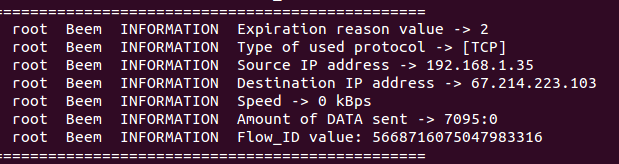
\includegraphics[width=0.9\textwidth]{konektivita_beem}
\caption{Test 1: Konektivita medzi exportérom a Mediátorom - strana exportéra}\label{o:konektivita_beem}
\end{figure}

\begin{figure}[ht!]
\centering
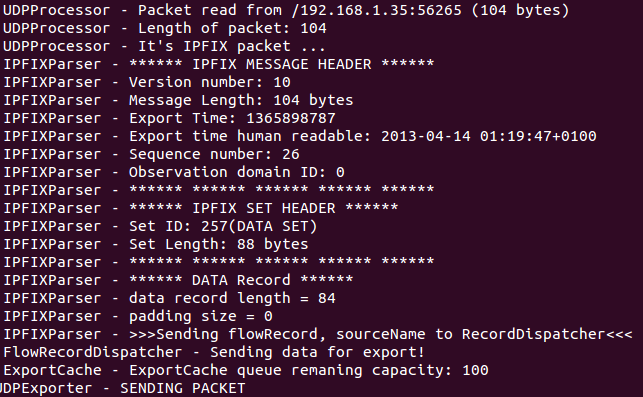
\includegraphics[width=0.9\textwidth]{konektivita_mediator}
\caption{Test 1: Konektivita medzi exportérom a Mediátorom - strana Mediátora}\label{o:konektivita_mediator}
\end{figure}

Konektivita medzi Mediátorom a kolektorom bola tiež potvrdená. Dôkazom boli logovacie výstupy kolektora, 
ktoré sú veľmi podobné ako tie z Mediátora. V databáze, na ktorú je JXColl pripojený, pribúdali správne 
záznamy. Tento experiment môžeme považovať za úspešný.

%%-------------------------

\subsection{Test správnej reprezentácie údajov}

Druhý experiment nadväzoval na predchádzajúci test konektivity. Testovacia topológia aj konfigurácie 
jednotlivých nástrojov boli rovnaké ako v predchádzajúcom prípade. V Mediátore stále neboli spustené 
žiadne sprostredkovateľské moduly. 

\begin{figure}[ht!]
\centering
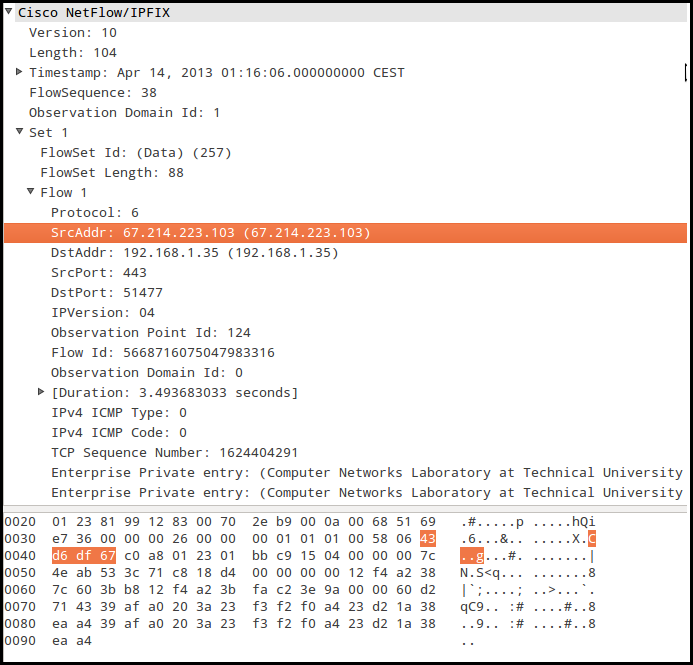
\includegraphics[width=1.0\textwidth]{porovnanie_wireshark}
\caption{Test 2: Správy odosielané exportérom zachytené programom Wireshark}\label{o:porovnanie_wireshark}
\end{figure}

\begin{figure}[ht!]
\centering
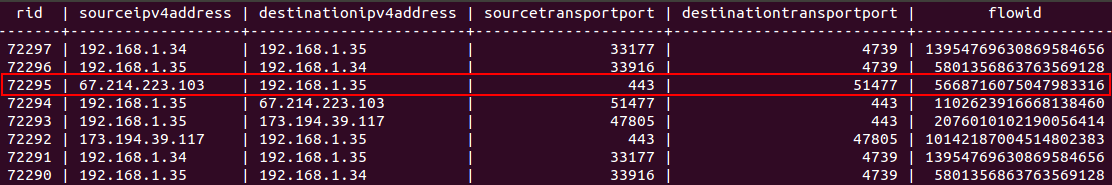
\includegraphics[width=1.0\textwidth]{porovnanie_db}
\caption{Test 2: Výpis obsahu databázy}\label{o:porovnanie_db}
\end{figure}

Myšlienkou tohto overenia bolo porovnať dáta, ktoré posiela exportér s dátami, ktoré prejdú celou topológiou
cez Mediátor a JXColl a sú uložené v databáze. Na zachytenie správ z mybeem-u bol použitý program 
Wireshark, ktorý odchytával sieťovú prevádzku na prvom počítači, na rozhraní \emph{eth0} s IP adresou 
\emph{192.168.1.35}. Detail jednej zo správ, ktoré zachytil Wireshark je na Obrázku 
\ref{o:porovnanie_wireshark}. Na Obrázku \ref{o:porovnanie_db} sú zase vyfiltrované posledné záznamy, 
ktoré boli uložené do databázy. Môžeme porovnať aspoň na niekoľkých znázornených informačných elementoch,
že záznamy o toku sa po prechode cez topológiu s Mediátorom bez zapnutých sprostredkovateľských procesov 
nezmenili. Tento experiment považujeme za úspešný.

%%-------------------------

\subsection{Test Mediátora s anonymizačným modulom}

Tento experiment je miernou úpravou predchádzajúceho. Testovacia topológia aj konfigurácie nástrojov boli 
rovnaké s tým rozdielom, že v Mediátore bol zapnutý jednoduchý anonymizačný proces - \verb|ExampleProcess|.
Tento modul bol naprogramovaný kvôli demonštrácii implementácie sprostredkovateľského procesu. Cieľom 
experimentu bolo dokázať dve tvrdenia:
\begin{itemize}
 \item Aplikačný rámec poskytuje sprostredkovateľským procesom správne metódy na dekódovanie a zakódovanie
 dátových záznamov. To platí vtedy, keď hodnoty informačných elementov sa rovnajú hodnotám záznamov
 v databáze po prechode celou topológiou aj keď sú spustené sprostredkovateľské moduly.
 \item Anonymizačný modul správne modifikuje zdrojovú a cieľovú IP adresu toku. Výsledkom je to, že 
 posledný oktet je v obidvoch prípadoch nahradený nulou.
\end{itemize}

\begin{figure}[ht!]
\centering
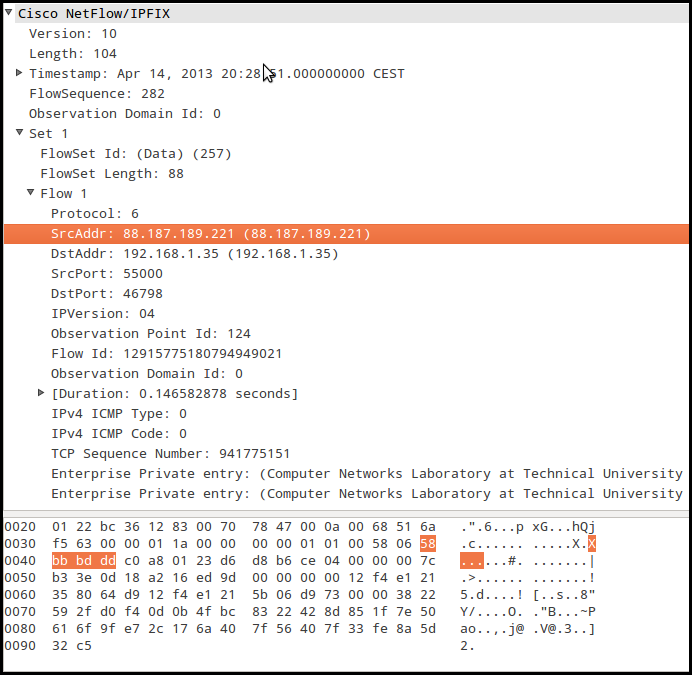
\includegraphics[width=1.0\textwidth]{anonym_wireshark}
\caption{Test 3: Správy odosielané exportérom zachytené programom Wireshark}\label{o:anonym_wireshark}
\end{figure}

\begin{figure}[ht!]
\centering
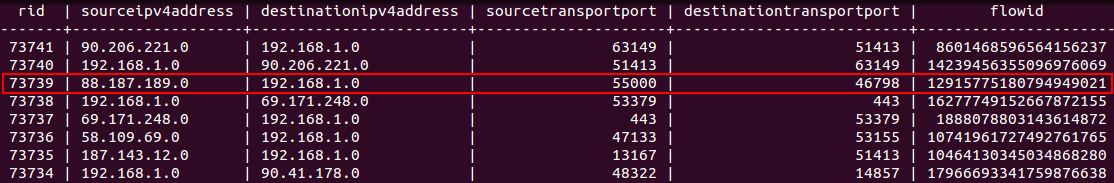
\includegraphics[width=1.0\textwidth]{anonym_db}
\caption{Test 3: Výpis obsahu databázy}\label{o:anonym_db}
\end{figure}


Na Obrázku \ref{o:anonym_wireshark} je zobrazený detail jednej zo správ, ktorú exportoval mybeem. 
Na nasledujúcom Obrázku \ref{o:anonym_db} vidieť posledne záznamy z databázy. Môžeme porovnať, že hodnoty 
zdrojového a cieľového transportného portu a hodnota \emph{flowId} sa nezmenili. Avšak zároveň, všetky 
zdrojové a cieľové IP adresy boli anonymizované. Tento experiment považujeme za úspešný, dokázal správnosť 
obidvoch tvrdení.


\subsection{Záťažový test}





